%! Author = Philipp Emmenegger
%! Date = 30/06/2021

\section{Application Protocols}
\textbf{Designing custom protocols}\\
- Needs more time to develop / test\\
+ Can be more efficient (space/performance)\\
\textbf{Protocol generators:} (ASN1, ProtoBuf)\\
+ IDL (interface description language) generates code\\
+ Standard\\
- Has more overhead\\

\subsection{ASN1}
\begin{itemize}
    \item Define data structures
    \item Can be serialized and deserialized
    \item Generic binary protocol
\end{itemize}

\subsection{Protocol Buffers (ProtoBuf)}
\begin{itemize}
    \item Data serialization system from Google
    \item Design goals: smaller and faster than XML
    \item Use: nearly all inter-machine communication at Google
    \item Contains only numbers, not field names
\end{itemize}

\subsection{gRPC}
\begin{itemize}
    \item Uses HTTP/2 for transport
    \item Uses ProtoBuf
    \item Features
    \begin{itemize}
        \item Authentication
        \item Bidirectional Streaming
        \item Flow Control
        \item Blocking / Nonblocking bindings
        \item Cancellation and timeouts
    \end{itemize}
    \item Define services and messages
\end{itemize}

\subsection{JSON + REST}
\begin{itemize}
    \item Human readable text to transmit data
    \item Often used for web apps
    \item Parsing overhead
    \item JSON slower than binary protocol
\end{itemize}

\subsection{HTTP}
\begin{itemize}
    \item Text based protocol
    \item Request / Response
    \item Request Methods
    \begin{itemize}
        \item GET, HEAD, POST, PUT, DELETE, TRACE, OPTIONS, CONNECT, PATCH
    \end{itemize}
    \item Stateless
    \item HTTP resources identified by URL
\end{itemize}
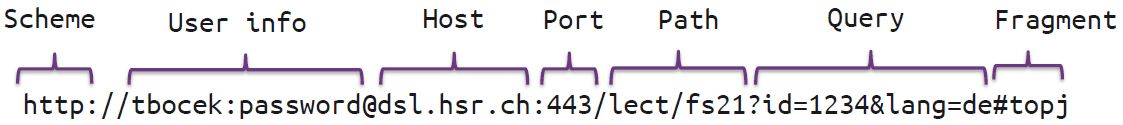
\includegraphics[width=\linewidth]{../img/http.png}

\subsection{DNS}
\begin{itemize}
    \item Translates human readable domain to IP
    \item Phonebook of the Internet
    \item Hierarchical and decentralized naming system
    \item Caching/forwarding DNS
    \item Recursive servers
    \item Authoritative servers
    \item Restriction to 13 root servers (512 byte packet limit)
\end{itemize}
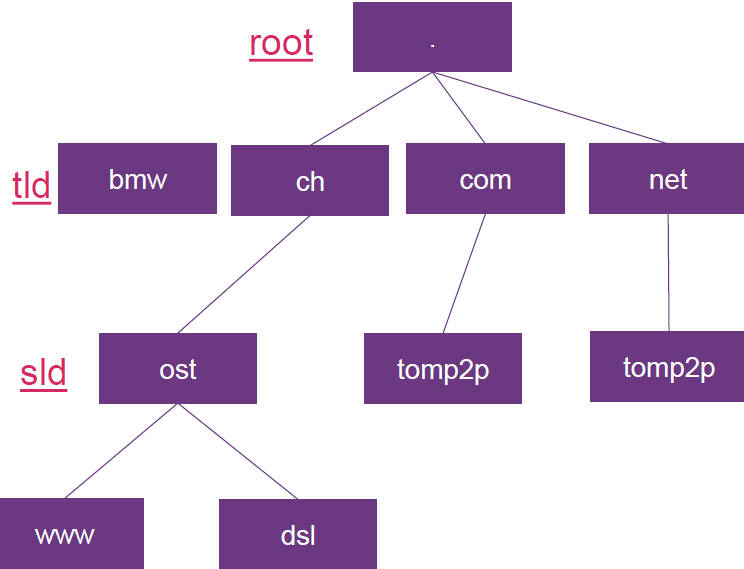
\includegraphics[width=\linewidth]{../img/dns.png}
\textbf{Type of records:}
\begin{itemize}
    \item SOA: Start of Authority
    \item NS
    \item MX
    \item A/AAAA
    \item TXT
    \item PTR
\end{itemize}
\textbf{DNSSEC}
\begin{itemize}
    \item Authenticated and data integrity, NOT confidentiality
    \item Can be used to bootstrap other security systems
    \item KSK: key singing keys to sign ZSK
    \item ZSK: zone signing keys to sign records
\end{itemize}

\subsubsection{The DNS war}
\textbf{DoH (DNS over HTTP)}
\begin{itemize}
    \item Provides confidentiality of lookups in transit
    \item Uses standard HTTP/2 on Port 443
    \item Trivially deployed, DNS response served like web pages
    \item Performance: TCP+TLS handshake = 2/3 RTT
    \item Difficult upgrade path for clients
    \item Browsers can perform DNS queries using JavaScript
\end{itemize}
\textbf{DoT (DNS over TLS)}
\begin{itemize}
    \item Provides confidentiality of lookups in transit
    \item DNS over TLS, separate port 853, can be blocked
    \item Widely supported by serving software and public resolvers
    \item Performance: TCP+TLS handshake = 2/3 RTT
    \item Easy upgrade path for clients
\end{itemize}

\subsection{Let's Encrypt}
\begin{itemize}
    \item Non-profit CA
    \item Provides certificates for TLS
    \item No Identity Checks
    \item Certificates are valid for 90 days
    \item Automated renewal
    \begin{itemize}
        \item ACME protocol: challenge response
    \end{itemize}
\end{itemize}